\documentclass{article}
\usepackage{graphicx}
\usepackage{amsmath}
\usepackage{booktabs} % For better table lines
\usepackage{adjustbox} % To fit table if needed
% Packages for enhanced functionality
\usepackage{graphicx}      % For including images
\usepackage{caption}       % For customizing captions
\usepackage{amsmath}       % For mathematical symbols and environments
\usepackage{geometry}      % To adjust page margins
\usepackage{float}         % For improved figure placement
\usepackage{hyperref}      % For hyperlinks within the document

\title{Project 1 - Question 2 - Part 1}
\author{Adil Hydari}
\date{\today}
\begin{document}
	
	\maketitle
	\section{Lab 1}
	\subsection{Part 1}
	
	\begin{table}[ht]
		\centering
		\begin{adjustbox}{max width=\textwidth}
			\begin{tabular}{|l|c|c|c|c|c|c|c|}
				\hline
				\textbf{Benchmark}      & \textbf{Total \# of Instructions} & \textbf{Load \%} & \textbf{Store \%} & \textbf{Uncond Branch \%} & \textbf{Cond Branch \%} & \textbf{Integer Computation \%} & \textbf{Floating pt Computation \%} \\ \hline
				anagram.alpha           &25,597,771&25.36&9.93&4.46&10.30&44.63&5.31 \\ \hline
				go.alpha                &545,812,145&30.62&8.17&2.58&10.96&47.64&0.03 \\ \hline
				compress.alpha          &88,337&1.66&79.05&0.19&5.78&13.30&0.00      \\ \hline
				gcc.alpha               &337,341,325& 24.67&11.47&4.12&13.33&46.30&0.11 \\ \hline
			\end{tabular}
		\end{adjustbox}
		\caption{Instruction breakdown for given benchmarks}
	\end{table}
	
\subsection{Part 2}
	\begin{table}[ht]
	\centering
	\begin{adjustbox}{max width=\textwidth}
		\begin{tabular}{|l|c|c|c|c|c|c|c|}
			\hline
			\textbf{Alpha Benchmark}      & \textbf{Total \# of Instructions} & \textbf{Load \%} & \textbf{Store \%} & \textbf{Uncond Branch \%} & \textbf{Cond Branch \%} & \textbf{Integer Computation \%} & \textbf{Floating pt Computation \%} \\ \hline
			test.math          &49,604&17.24&10.38&3.92&11.16&55.27&1.87 \\ \hline
			test.fmath                &19,693&17.88&12.40&4.65&11.50&53.00&0.42 \\ \hline
			test.llong          &10,821&18.09&14.33&5.32&12.78&49.19&0.10      \\ \hline
			test-printf               &983,667& 18.00&10.73&4.82&11.39&54.84&0.09 \\ \hline
		\end{tabular}
	\end{adjustbox}
	\caption{Instruction breakdown for Alpha benchmarks}
\end{table}

\begin{table}[ht]
	\centering
	\begin{adjustbox}{max width=\textwidth}
		\begin{tabular}{|l|c|c|c|c|c|c|c|}
			\hline
			\textbf{Pisa Benchmark}      & \textbf{Total \# of Instructions} & \textbf{Load \%} & \textbf{Store \%} & \textbf{Uncond Branch \%} & \textbf{Cond Branch \%} & \textbf{Integer Computation \%} & \textbf{Floating pt Computation \%} \\ \hline
			test.math          &213,745&15.96&10.66&4.22&13.85&54.42&0.88 \\ \hline
			test.fmath                &53,504&16.14&14.41&4.24&15.11&49.95&0.11 \\ \hline
			test.llong          &29,687&16.33& 17.99&4.37&15.45&45.82&0.00      \\ \hline
			test-printf               &1,813,937&19.22&9.28&5.13&17.01&49.33&0.01 \\ \hline
		\end{tabular}
	\end{adjustbox}
	\caption{Instruction breakdown for Pisa benchmarks}
\end{table}
\subsection{Comparison with Histogram}
\begin{figure}[H]
	\centering
	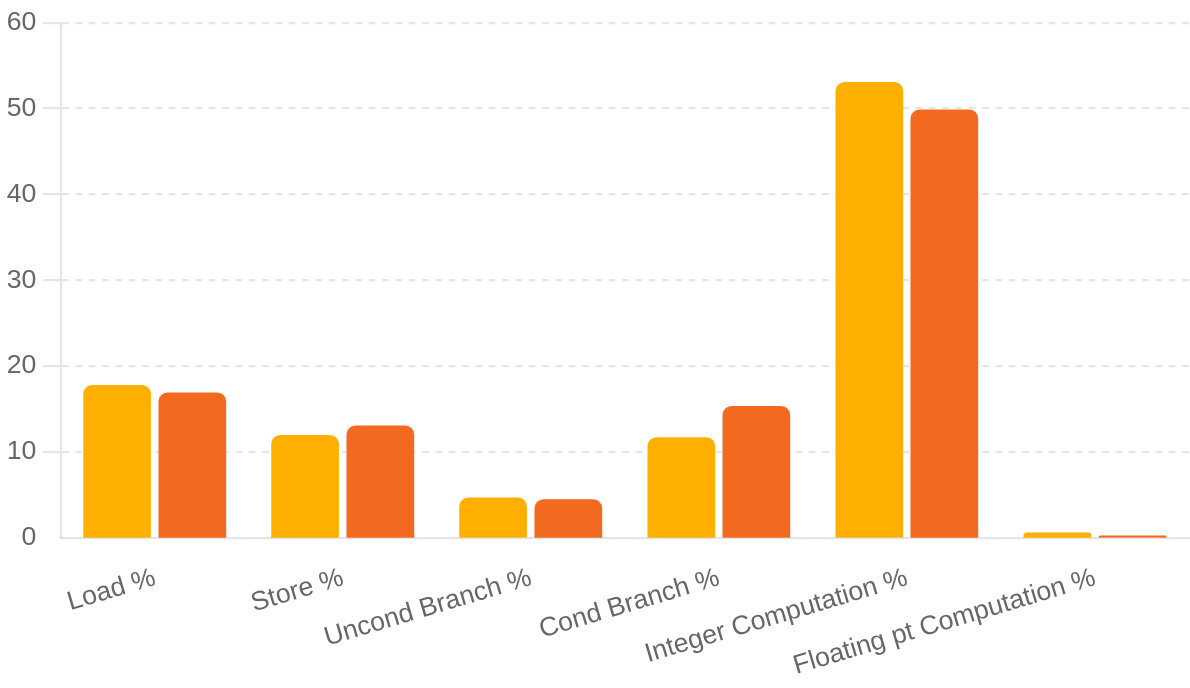
\includegraphics[width=\linewidth]{Comparison of Instruction Types Between Alpha and Pisa ISAs.png}
	\caption{Comparison of Instruction Types (Averages) Between Alpha and Pisa ISAs}
	\label{fig:memory_bandwidth}
\end{figure}
Seems like PISA generates a lot more instructions, compared to Alpha, from the compiler, this indicates that the perhaps PISA's MIPs implementation is more CISC like when compared to the Alpha ISA. 

\section{Lab 6}
\subsection{Tests}

\begin{figure}[H]
	\centering
	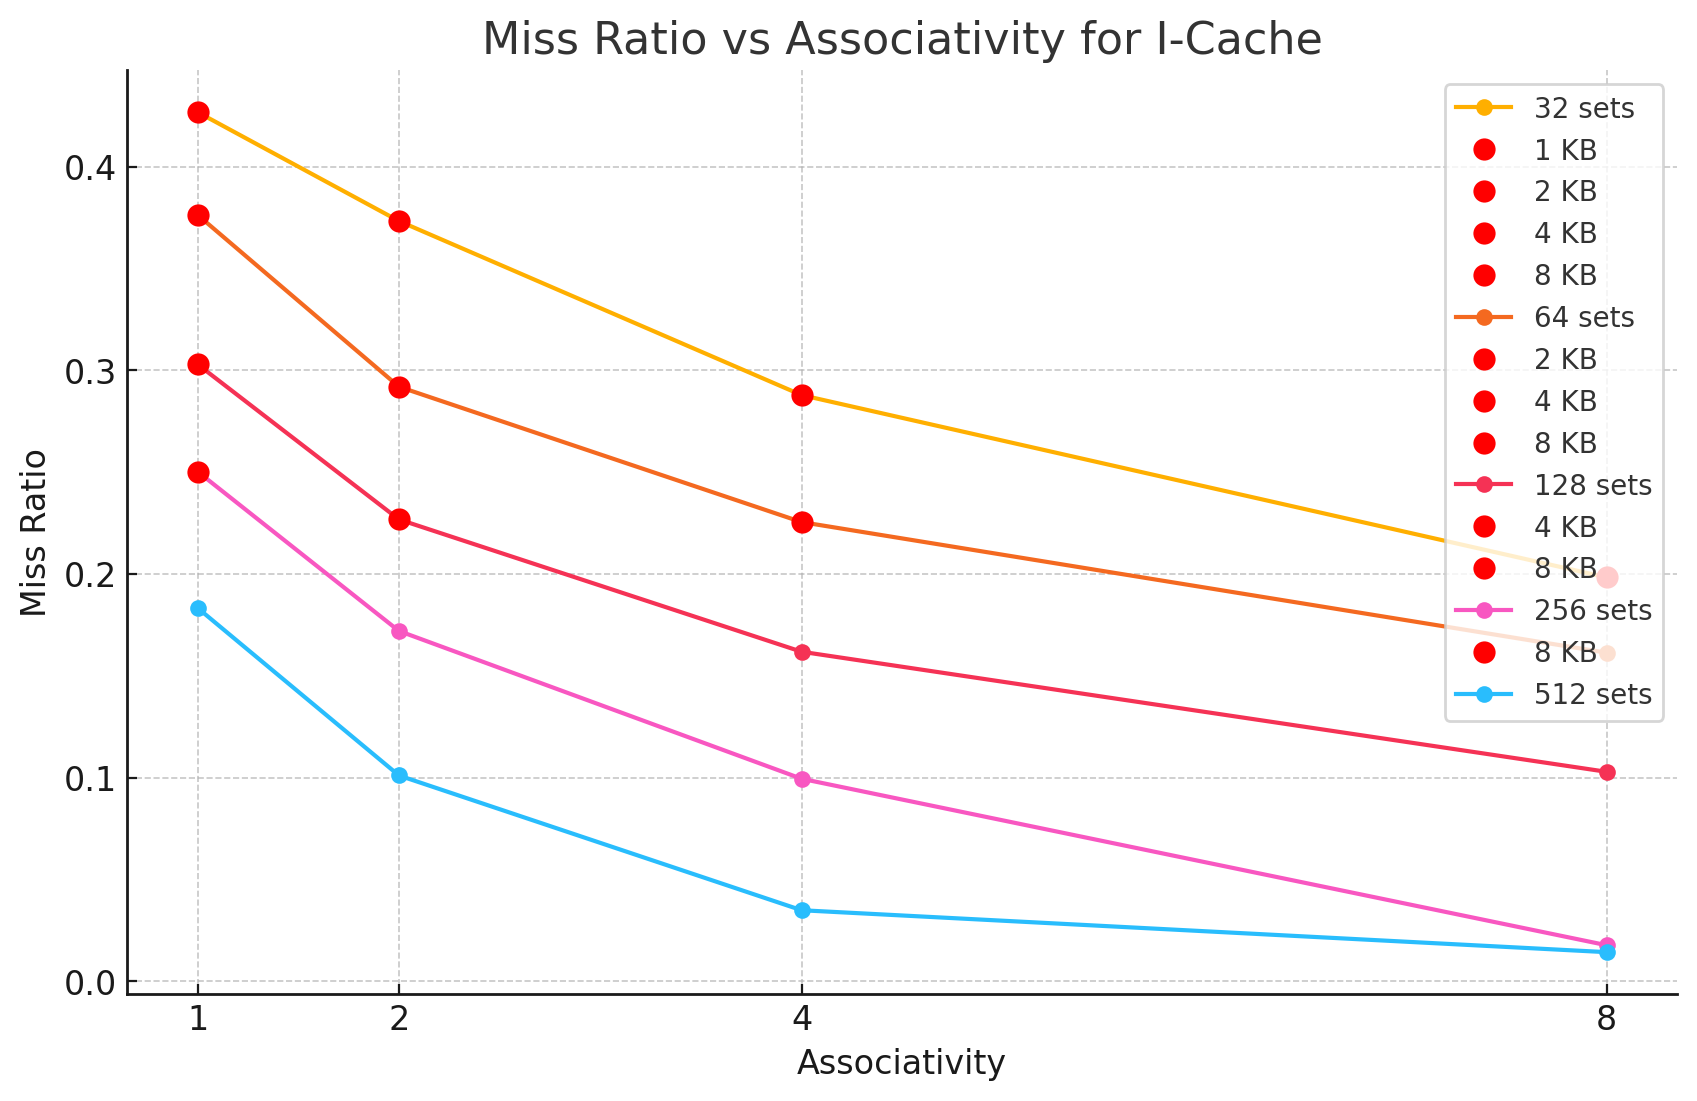
\includegraphics[width=\linewidth]{icache.png}
	\caption{Miss Ratio vs Associativity for I-Cache}
	\label{fig:icache}
\end{figure}
\begin{table}[h]
	\centering
	\begin{tabular}{|c|c|c|c|c|}
		\hline
		\textbf{Miss Ratio (I-Cache)} & \textbf{1-way} & \textbf{2-way} & \textbf{4-way} & \textbf{8-way} \\ \hline
		\textbf{32 sets}  &       0.4269      &       0.3734     &      0.2879       &       0.1983      \\ \hline
		\textbf{64 sets}  &        0.3764    &       0.2920     &       0.2255      &      0.1613      \\ \hline
		\textbf{128 sets} &       0.3030      &       0.2268     &        0.1618    &      0.1028       \\ \hline
		\textbf{256 sets} &        0.2503     &      0.1720       &      0.0994       &       0.0176      \\ \hline
		\textbf{512 sets} &       0.1833     &      0.1010      &       0.0348      &      0.0142      \\ \hline
	\end{tabular}
	\caption{Miss Ratio for I-Cache}
	\label{tab:I-Cache}
\end{table}


\begin{figure}[H]
	\centering
	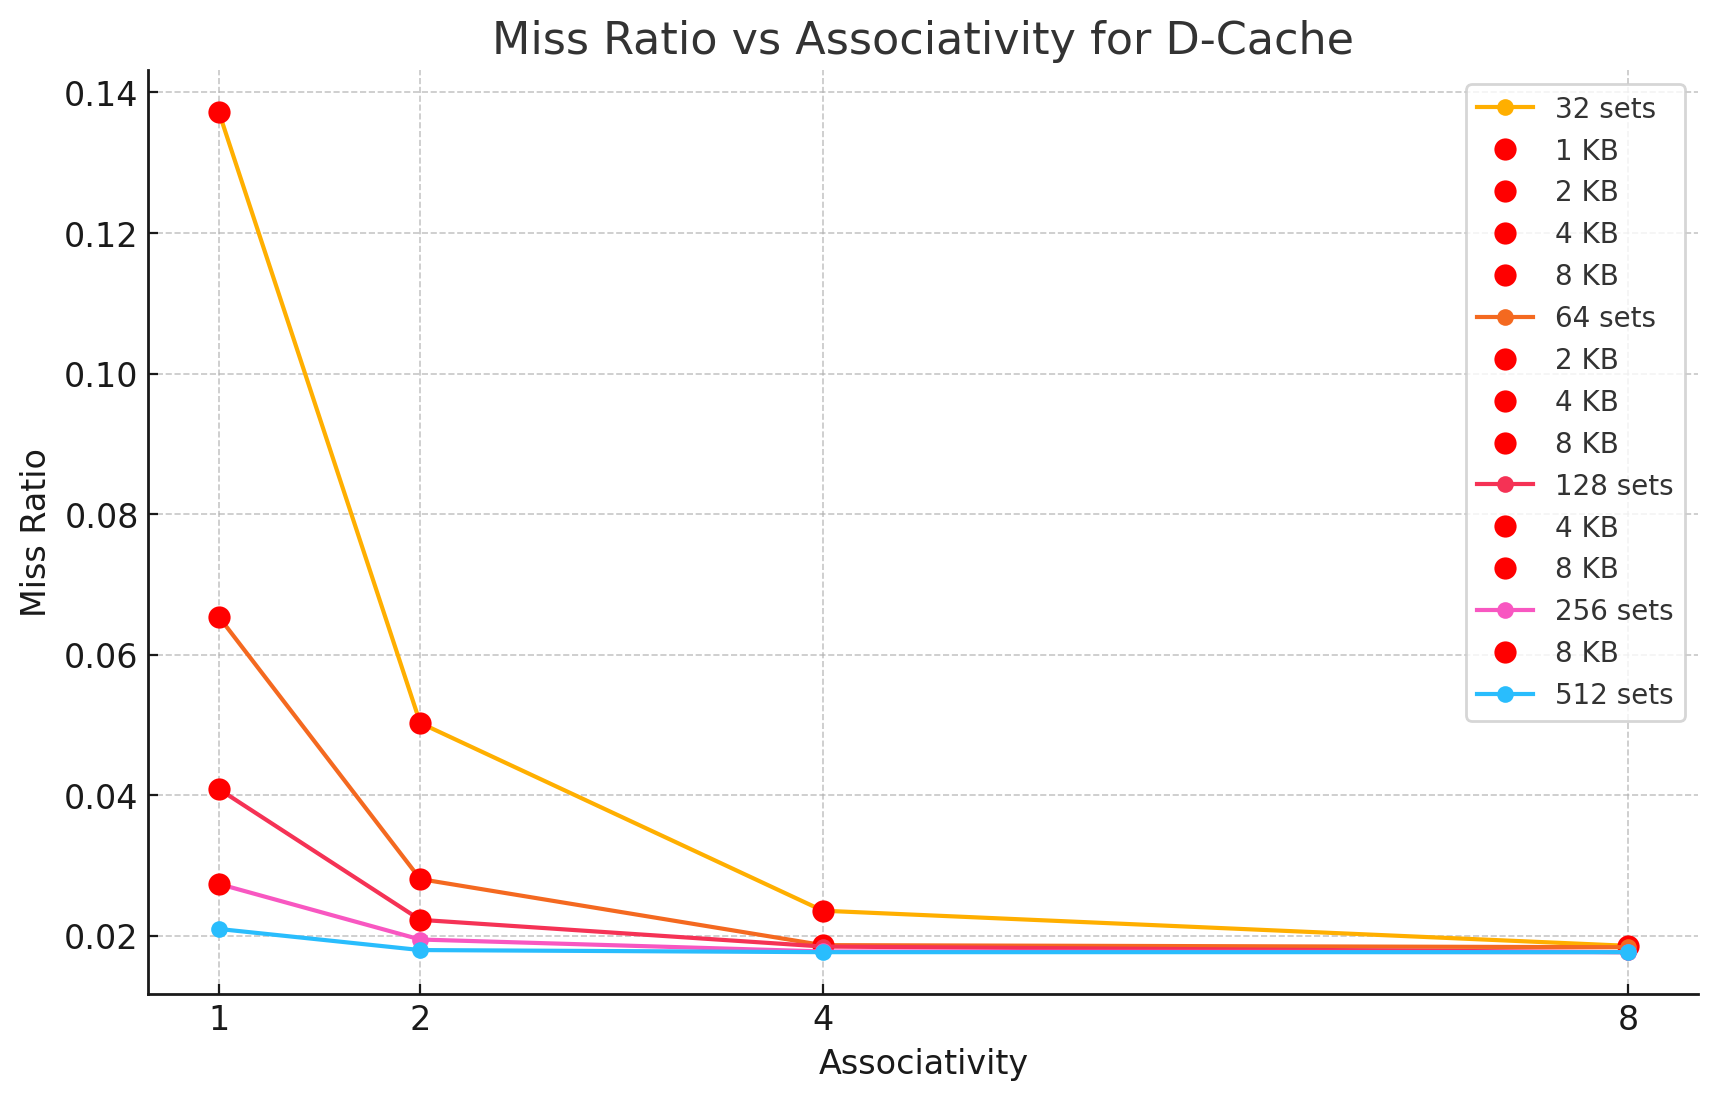
\includegraphics[width=\linewidth]{dcache.png}
	\caption{Miss Ratio vs Associativity for D-Cache}
	\label{fig:dcache}
\end{figure}


\begin{table}[h]
	\centering
	\begin{tabular}{|c|c|c|c|c|}
		\hline
		\textbf{Miss Ratio (D-Cache)} & \textbf{1-way} & \textbf{2-way} & \textbf{4-way} & \textbf{8-way} \\ \hline
		\textbf{32 sets}  &       0.1372    &     0.0503       &        0.0236      &     0.0186        \\ \hline
		\textbf{64 sets}  &      0.0654       &      0.0281       &     0.0187       &       0.0184      \\ \hline
		\textbf{128 sets} &      0.0409       &       0.0223      &      0.0185       &      0.0177       \\ \hline
		\textbf{256 sets} &       0.0274      &      0.0195       &      0.0178       &      0.0177        \\ \hline
		\textbf{512 sets} &      0.0210       &      0.0180       &      0.0177       &     0.0177        \\ \hline
	\end{tabular}
	\caption{Miss Ratio for D-Cache}
	\label{tab:D-Cache}
\end{table}

\subsection{Cache Simulation Analysis}

\subsubsection{Questions and Answers}

\textbf{Q1: For a given number of sets, what effect does increasing associativity have on the miss ratio?}

For a given number of sets, increasing associativity reduces the miss ratio. This is evident from the tables where, for each fixed number of sets, the miss ratio decreases as the associativity increases. Higher associativity allows more blocks to reside in the same set, reducing conflict misses caused by multiple blocks competing for the same cache location.

\textbf{Q2: For a given associativity, what is the effect of increasing the number of sets?}

For a given associativity, increasing the number of sets decreases the miss ratio. This is because increasing the number of sets effectively enlarges the cache size (since total cache size = number of sets $\times$ associativity $\times$ block size), allowing more unique blocks to be stored. This reduces capacity misses, as the cache can hold more data.

\textbf{Q3: For a given cache size, how does the miss ratio change when going from an associativity of one to two to four? Explain.}

For a given cache size, increasing associativity from one to two to four generally leads to a reduction in the miss ratio, but the improvement diminishes with higher associativity. This is because, while higher associativity reduces conflict misses by allowing more blocks per set, the total number of unique blocks that can be stored (cache capacity) remains the same. Therefore, the initial increase from direct-mapped (1-way) to 2-way associativity shows a noticeable improvement, but going from 2-way to 4-way yields smaller gains due to diminishing returns.

\textbf{Q4: If you were to design an Instruction cache, limited to a total cache size of 4 Kbytes, which cache organization would you choose, based solely on performance?}

For designing a 4 Kbytes instruction cache based solely on performance, the best choice is a \textbf{4-way set-associative cache with 32 sets}. This configuration offers the lowest miss ratio among the options with the same cache size (4 Kbytes). Here’s why:

\begin{itemize}
	\item Cache size = Number of sets $\times$ Associativity $\times$ Block size
	\item Assuming a block size of 32 bytes, the configurations that yield 4 Kbytes cache size are:
	\begin{itemize}
		\item 1-way, 128 sets
		\item 2-way, 64 sets
		\item 4-way, 32 sets
	\end{itemize}
	\item From the I-Cache table:
	\begin{itemize}
		\item 1-way, 128 sets: miss ratio = 0.3030
		\item 2-way, 64 sets: miss ratio = 0.2920
		\item \textbf{4-way, 32 sets: miss ratio = 0.2879 (lowest)}
	\end{itemize}
\end{itemize}

\textbf{Q5: If you were to design a data cache, limited to a total cache size of 4 Kbytes, which cache organization would you choose, based solely on performance?}

For designing a 4 Kbytes data cache based solely on performance, the optimal choice is also a \textbf{4-way set-associative cache with 32 sets}. This configuration provides the lowest miss ratio among the available options with the same cache size. Supporting data:

\begin{itemize}
	\item Cache size = Number of sets $\times$ Associativity $\times$ Block size
	\item Assuming a block size of 32 bytes, the configurations that yield 4 Kbytes cache size are:
	\begin{itemize}
		\item 1-way, 128 sets
		\item 2-way, 64 sets
		\item 4-way, 32 sets
	\end{itemize}
	\item From the D-Cache table:
	\begin{itemize}
		\item 1-way, 128 sets: miss ratio = 0.0409
		\item 2-way, 64 sets: miss ratio = 0.0281
		\item \textbf{4-way, 32 sets: miss ratio = 0.0236 (lowest)}
	\end{itemize}
\end{itemize}

	
\end{document}
